%Anie - ohkis.sourceforge.net
%Unai Martinez Corral
%umartinez012@ikasle.ehu.es
%
% <- anie.tex

\section{Sarrera}

2007 urtean zehar \emph{Iñaki Silanes}ek, \textbf{U}niversidad del \textbf{P}aís \textbf{V}asco \textbf{/} \textbf{E}uskal \textbf{H}erriko \textbf{U}nibertsitateko\footnote{\url{www.ehu.es}} \textbf{ITSAS}\footnote{\url{itsas.ehu.es}} Software Libre Taldeko kideak, \LaTeX{}\footnote{\url{en.wikipedia.org/wiki/LaTeX}} eta \emph{OpenDocument}\footnote{\url{en.wikipedia.org/wiki/OpenDocument}} formatuetan Unibertsitatean gazteleraz, euskaraz zein ingelesez Karrera Amaierako Proiektuak zein Doktorego Tesiak aurkezteko txantiloiak eskaintzeko helburuarekin \emph{Plantillas para Proyecto de Fin de Carrera} lan taldea\footnote{\url{itsas.ehu.es/workgroups/plantillas_proyecto_fin_de_carrera}} osatu zuen.

2010 urtean \emph{Digna González} eta \emph{Unai Martinez}ek lan talde berrian\footnote{\url{itsas.ehu.es/workgroups/latex}} \emph{Iñaki Silanes}en lana \emph{\LaTeX{}} erabiltzeko hainbat argibide, erreferentzia, aurkezpen eta abarrekin bateratu zuten eta material bera baliatuz zenbait ikastaro eman.

Idazleak, \textbf{Bi}lboko \textbf{I}ndustria \textbf{I}ngeniaritza \textbf{T}eknikoko \textbf{U}nibertsitate \textbf{E}skolan\footnote{\url{www.industria-ingeniaritza-tekniko-bilbao.ehu.es}} Karrera Amaierako Proiektua euskaraz idazteko orduan eskuragarri zeuden txantiloiek premia\footnote{\url{www.industria-ingeniaritza-tekniko-bilbao.ehu.es/p229-content/eu/contenidos/normativa/euiti_bi_pfc/eu_nor_gral/normativa_gral_fin_carrera.html}} guztiak asetzen ez zituztenez, aipatutako lan taldeetan bildutakoak oinarri, eskuartean duzun txantiloi berria egin du. \hyperref[tab:comp]{\ref*{tab:comp} taula}k \emph{Iñaki Silanes}ek eskainitakoekiko ezberdintasun nagusiak biltzen ditu.

\begin{table}[!htp]
\begin{tabular}{c c c c l}
& \bfseries Hizkuntza & \bfseries Formatua & \bfseries Klasea & \\
&&&&\\
\multirow{2}{*}{\bfseries Iñaki Silanes} & EU & \LaTeX{} & \multirow{2}{*}{\emph{itsas\_pfc.cls}} & \multirow{2}{*}{\emph{book} oinarri}\\
& ES EN & OpenDocument & & \\
&&&&\\
\bfseries Unai Martinez & EU & \LaTeX{} & \emph{report} & \emph{config} fitxategietan moldatuta\\
\end{tabular}
\caption{\emph{Iñaki Silanes}en txantiloiekin konparaketa.}
\label{tab:comp}
\end{table}

Horietaz gain, hurrengo berrikuntzak ditu honek:

\begin{itemize}
\item{Kapitulu, atal, azpiatal, azpiazpiatal, irudi eta taulak zenbakitu eta izendatzean zenbakia azaltzen da lehenengo, puntu ordinala ondoren eta hitza azkenik.}
\item{\emph{babel}ek \emph{basque} aukeratzean ezatzen duen data komandoaren ordez \emph{gaur} sortu da.}
\item{\emph{Kapitulu}en izen gisa \emph{Dokumentu} ezarri da.}
\item{BI-IITUEko web gunean soilik DOC formatuan eskuragarri dauden txantiloiak erabili dira \emph{Kapitulu/Dokumentu}en portadak diseinatzeko.}
\item{Atalen goiburuak aldatu dira.}
\item{Ikurren Zerrenda gehitu da.}
\item{BI-IITUEko arautegiak eskatu bezala, \emph{UNE 157001-2002} araua erreferentzia izanik banatu da edukia. Hala ere, txantiloi honek ez du araua betetzen. Karrera Amaierako Proiektuen helburu nagusia hezkuntza eta ikastea izanik, edukia aurkitzea eta dokumentuen banakako azterketa errazteko diseinuan zenbait erabaki ezberdin hartu dira:
 \begin{itemize}
  \item{Dokumentuen ordena aldatu da eta zenbait ezabatu.}
  \item{Portadak ez daude zenbakituta.}
  \item{Orrialde, irudi, taula eta ekuazioen zenbakitzea kapitulu bakoitzean berrabiatzen da.} 
  \item{Zenbakitzea 0an hasten da.}
  \item{Aurkibideen orrialdeak zenbaki erromatarrez daude adierazita.}
  \item{Eranskinen dokumentuan atalak alfabetoz izendatzen dira.}
  \item{Goiburu eta orri oinen edukiak tokiz aldatuta daude eta dokumentu, atal zein azpiatalen arabera berritzen dira.}
 \end{itemize}
Hau dela eta, araua betetzeko \emph{config} karpetako fitxategietan moldaketak egin behar ditu txantiloiaren erabiltzaileak.
}
\end{itemize}

Txantiloia erabiltzeko argibideak (fitxategien antolaketa, moldaketen izaera, etab.) \hyperref[att:atta]{\ref*{att:atta} eranskin}ean eta \hyperref[att:attb]{\ref*{att:attb} eranskin}ean aurkitu daitezke.

Edozein kasutan, emaitza zuzena izan dadin hainbat aldiz konpilatu behar da lana, hurrengo ordena jarraituz:

\begin{center}
\Large\bfseries
PDFLaTeX + BibTeX + PDFLaTeX + PDFLaTeX
\end{center}

Atal eta azpiataletan aldaketa asko egitean, tarte fitxategiak edo fitxategi laguntzaileak (\emph{.aux}, \emph{.mtc}, \emph{.mlf}, \emph{.mlt}, etab.) ezabatzea komeni da, aurreko katea exekutatu baino lehen.

\bigskip

Adibide den txosten honetan zehar, garapenean zehar erabilitako zenbait baliabide tartekatuko dira, ideiak hartzeko balioko dutelako itxaropenez. \hyperref[fig:ychart]{\ref*{fig:ychart} irudia}k adierazten duen grafikoa, esaterako. Irudi guztien kodea txantiloien iturrietan dago, \emph{TikZ/PGF}\footnote{\url{texample.net/tikz/examples}} paketeak baliatuz egin baitira.

\begin{figure}[!htp]
\centering
%% Copyright 2009 Ivan Griffin
%
% This work may be distributed and/or modified under the
% conditions of the LaTeX Project Public License, either version 1.3
% of this license or (at your option) any later version.
% The latest version of this license is in
%   http://www.latex-project.org/lppl.txt
% and version 1.3 or later is part of all distributions of LaTeX
% version 2005/12/01 or later.
%
% This work has the LPPL maintenance status `maintained'.
% 
% The Current Maintainer of this work is Ivan Griffin
%
% This work consists of the files y_chart_common.tex and y_chart_example.tex

%Description
%-----------
%y_chart_common.tex -  TikZ code to draw the 3 axes of the 
%                      Gajski-Kuhn Y-chart
%y_chart_example.tex - an example file which connects and describes
%                      the Y-chart

%Created 2009-11-20 by Ivan Griffin.  Last updated: 2009-11-20
%-------------------------------------------------------------

 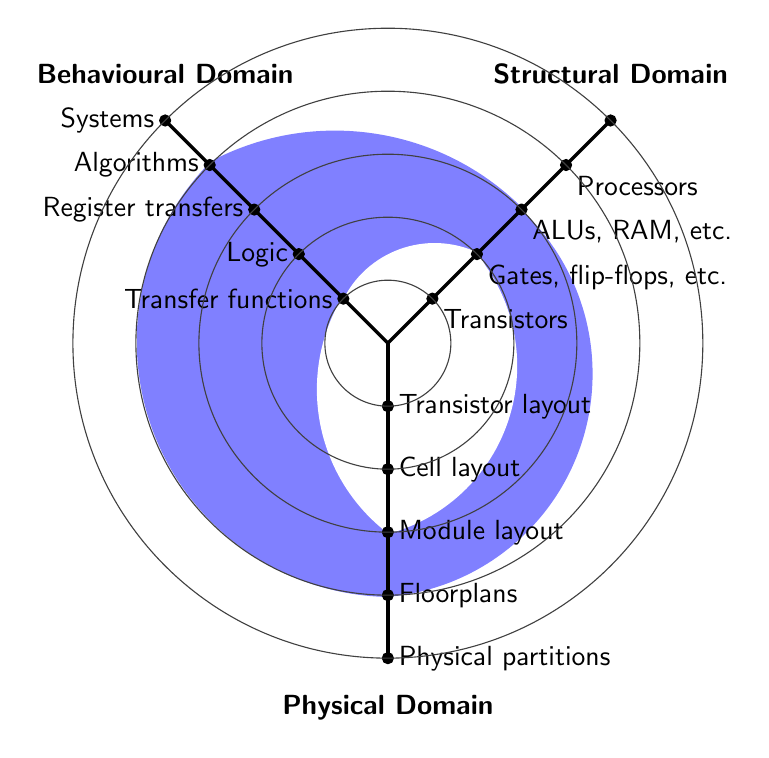
\begin{tikzpicture}[>=stealth,join=bevel,font=\sffamily,auto]
    \coordinate (behaviouralNode) at (135:4cm);
    \coordinate (structuralNode) at (45:4cm);
    \coordinate (physicalNode) at (270:4cm);
    \coordinate (originNode) at (0:0cm);

\draw[very thick,blue!50,fill=blue!50] (barycentric cs:physicalNode=0.8,originNode=0.2) arc (-85:50:2.825) -- (barycentric cs:structuralNode=0.6,originNode=0.4) arc (45:117.5:3.3525) -- (barycentric cs:behaviouralNode=0.8,originNode=0.2) arc (136:267.5:3.225) -- cycle; 
\draw[very thick,white,fill=white] (barycentric cs:physicalNode=0.6,originNode=0.4) arc (-75:35:2.1875) -- (barycentric cs:structuralNode=0.4,originNode=0.6) arc (65:250:1.275) -- (barycentric cs:behaviouralNode=0.2,originNode=0.8) arc (149.5:230:2.275) -- cycle; 

%\draw[very thick,blue!25,fill=blue!50] (barycentric cs:physicalNode=0.8,originNode=0.2) -- (barycentric cs:structuralNode=0.6,originNode=0.4) -- (barycentric cs:behaviouralNode=0.8,originNode=0.2) -- cycle;
%\draw[very thick,blue!25,fill=white] (barycentric cs:physicalNode=0.6,originNode=0.4) -- (barycentric cs:structuralNode=0.4,originNode=0.6) -- (barycentric cs:behaviouralNode=0.4,originNode=0.6) -- cycle;

    \node [above=1em] at (behaviouralNode) {\textbf{Behavioural Domain}};
    \node [above=1em] at (structuralNode) {\textbf{Structural Domain}};
    \node [below=1em] at (physicalNode) {\textbf{Physical Domain}};

    \draw[-, very thick] (behaviouralNode.south) -- (0,0) node[left,pos=0]{Systems} node[left,pos=0.2]{Algorithms} node[left,pos=0.4]{Register transfers} node[left,pos=0.6]{Logic} node[left,pos=0.8]{Transfer functions};

    \draw[-, very thick] (structuralNode.south) -- (0,0) node[pos=0]{ } node[pos=0.2]{Processors} node[pos=0.4]{ALUs, RAM, etc.} node[pos=0.6]{Gates, flip-flops, etc.} node[pos=0.8]{Transistors};

    \draw[-, very thick] (physicalNode.south) -- (0,0) node[right,pos=0]{Physical partitions} node[right,pos=0.2]{Floorplans} node[right,pos=0.4]{Module layout} node[right,pos=0.6]{Cell layout} node[right,pos=0.8]{Transistor layout};

    \draw[fill] (barycentric cs:behaviouralNode=1.0,originNode=0) circle (2pt);
    \draw[fill] (barycentric cs:behaviouralNode=0.8,originNode=0.2) circle (2pt);
    \draw[fill] (barycentric cs:behaviouralNode=0.6,originNode=0.4) circle (2pt);
    \draw[fill] (barycentric cs:behaviouralNode=0.4,originNode=0.6) circle (2pt);
    \draw[fill] (barycentric cs:behaviouralNode=0.2,originNode=0.8) circle (2pt);

    \draw[fill] (barycentric cs:structuralNode=1.0,originNode=0) circle (2pt);
    \draw[fill] (barycentric cs:structuralNode=0.8,originNode=0.2) circle (2pt);
    \draw[fill] (barycentric cs:structuralNode=0.6,originNode=0.4) circle (2pt);
    \draw[fill] (barycentric cs:structuralNode=0.4,originNode=0.6) circle (2pt);
    \draw[fill] (barycentric cs:structuralNode=0.2,originNode=0.8) circle (2pt);

    \draw[fill] (barycentric cs:physicalNode=1.0,originNode=0) circle (2pt);
    \draw[fill] (barycentric cs:physicalNode=0.8,originNode=0.2) circle (2pt);
    \draw[fill] (barycentric cs:physicalNode=0.6,originNode=0.4) circle (2pt);
    \draw[fill] (barycentric cs:physicalNode=0.4,originNode=0.6) circle (2pt);
    \draw[fill] (barycentric cs:physicalNode=0.2,originNode=0.8) circle (2pt);

    \draw[black!75] (0,0) circle (4.0cm);
    \draw[black!75] (0,0) circle (3.2cm);
    \draw[black!75] (0,0) circle (2.4cm);
    \draw[black!75] (0,0) circle (1.6cm);
    \draw[black!75] (0,0) circle (0.8cm);

  \end{tikzpicture}
\caption{Gajski-Kuhn Y-grafikoan proiektuaren abstrakzio maila.} 
\label{fig:ychart}
\end{figure}